\section{Остовное дерево связного графа. Минимальное остовное дерево. Алгоритмы Прима и Краскала, 
их применение.}

\begin{definition}
    \textit{Остовным (стягивающим) деревом} связного графа называется
    его подграф, содержащий все вершины графа и являющийся деревом.
\end{definition}

\begin{definition}
    Если каждому ребру графа сопоставляется какое-то число
    (называют вес или длина или стоимость ребра), то такой граф называется
    \textit{нагруженным (взвешенным) графом}.
\end{definition}

Обозначение: $l(e)$ -- длина ребра, $w(e)$ -- вес ребра.

Пример нагруженного графа и его остовного дерева
\begin{figure}[h]
    \centering
    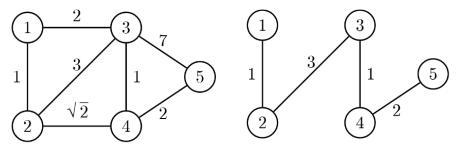
\includegraphics[scale=0.4]{25_1.png}
\end{figure}

Пусть $G$ -- нагруженный граф.

\begin{definition}
    \textit{Минимальным остовным деревом нагруженного графа}
    называется остовное дерево с минимальной суммой длин входящих в него
    ребер.
\end{definition}

Опишем алгоритмы Прима и Краскала, которые позволяют находить
минимальное остовное дерево нагруженного графа.

Алгоритмы Прима и Краскала называются также \textit{жадными алгоритмами}, то
есть алгоритмами, при которых на каждом шаге происходит поиск
оптимального выбора.

\textbf{Алгоритм Прима нахождения минимального остовного дерева.}
Пусть в нагруженном графе $G$ число вершин равно $n$.
\begin{enumerate}[left=0.0em, labelsep=1em, topsep=0.0em, itemsep=0pt, parsep=0.5em]
    \item Берем произвольную вершину графа. Находим в графе $G$ ребро
    минимальной длины, инцидентное этой вершине. Получаем подграф,
    состоящий из 2 вершин и ребра, соединяющего эти вершины. Обозначим этот
    подграф $G_2$, $i:=2$.
    \item Если $i=n$, то останавливаемся. Если нет, то переходим к шагу 3.
    \item Рассмотрим рёбра графа $G$, одна из вершин которых принадлежит
    графу $G_i$, а вторая не принадлежит. Из всех таких рёбер выбираем ребро
    минимальной длины и добавляем его к графу $G_i$. Получаем граф $G_{i+1}$, $i:=i+1$.
    Переходим к шагу 2.
\end{enumerate}

Пример. Найдем минимальное остовное дерево с помощью алгоритма Прима:
\begin{figure}[h]
    \centering
    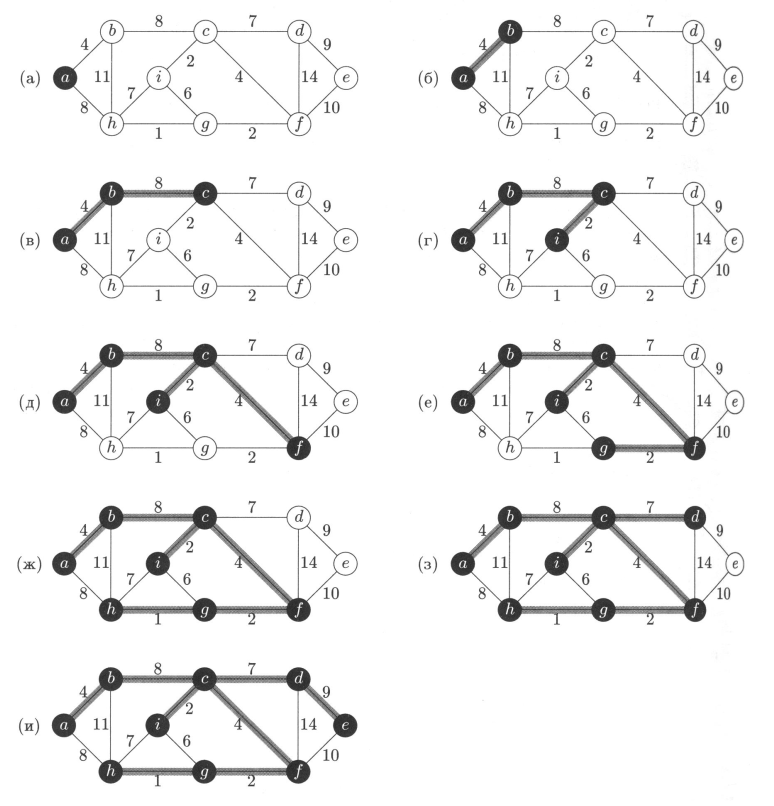
\includegraphics[scale=0.40]{25_2.png}
\end{figure}

Найдем длину(вес) полученного остовного дерева:

$4+8+7+9+2+4+1+2=37$

\newpage
\textbf{Алгоритм Краскала (Крускала) нахождения минимального остовного
дерева.}

Пусть в нагруженном графе $G$ число вершин равно $n$.
\begin{enumerate}[left=0.0em, labelsep=1em, topsep=0.0em, itemsep=0pt, parsep=0.5em]
    \item Упорядочиваем все ребра графа $G$ в порядке неубывания -- от ребер
    минимальной длины к максимальной. Множество ребер остовного дерева
    пусто.
    \item Первое ребро в остовном дереве - первое из упорядоченного списка (то
    есть ребро минимальной длины).
    \item Если в множестве ребер содержится $n-1$ ребер, то останавливаемся.
    Если нет, то переходим к шагу 4.
    \item Добавим в множество ребер остовного дерева такое ребро
    минимальной длины из оставшихся ребер, при добавлении которого не
    появятся циклы. Переходим к шагу 3.
\end{enumerate}

Пример. Найдем минимальное остовное дерево с помощью алгоритма
Краскала:
\begin{figure}[h]
    \centering
    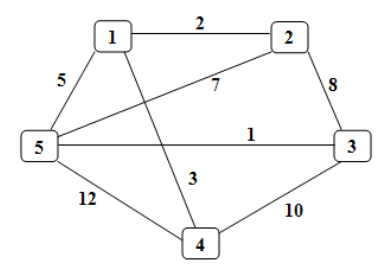
\includegraphics[scale=0.35]{25_3.png}
\end{figure}
\begin{enumerate}[left=0.0em, labelsep=1em, topsep=0.0em, itemsep=0pt, parsep=0.5em]
    \item Упорядочиваем ребра: $(5,3), (1,2), (1,4), (1,5), (5,2), (2,3), (3,4), (5,4)$.
    \item $V$ -- множество вершин, $E$ -- множество ребер остовного дерева. $V=\varnothing,E=\varnothing$.
    \item $E = \set{(5,3)}, V = \set{5,3}$
    \item $E = \set{(1,2), (5,3)}, V = \set{1,2,5,3}$
    \item $E = \set{(1,2), (5,3), (1,4)}, V = \set{1,2,5,3,4}$
    \item $E = \set{(1,2), (5,3), (1,4), (1,5)}, V = \set{1,2,5,3,4}$
    \item $n-1$ ребер, stop.
\end{enumerate}

Найдем длину (вес) полученного остовного дерева: $1+2+3+5=11$.